\documentclass[]{jarticle}          % 一段組
%\documentclass[twocolumn]{jarticle} % 二段組

\textwidth 180mm
\textheight 255mm
\oddsidemargin -12mm
\topmargin -15mm
\columnsep 10mm

%\vspace{0.5cm} % 一段組の場合はコメントアウトした方が体裁がよいx
%] % 一段組の場合はコメントアウトする

\usepackage{styles/labheadings}
\usepackage[dvipdfmx]{graphicx,color}
\usepackage{amsmath,amssymb}
\usepackage{url}
% 追加
\usepackage[hang,small,bf]{caption}
\usepackage[subrefformat=parens]{subcaption}
\captionsetup{compatibility=false}

\newcommand{\aU}{\mbox{\boldmath $a$}}
\newcommand{\bU}{\mbox{\boldmath $b$}}
\newcommand{\cU}{\mbox{\boldmath $c$}}
\newcommand{\dU}{\mbox{\boldmath $d$}}
\newcommand{\eU}{\mbox{\boldmath $e$}}
\newcommand{\fU}{\mbox{\boldmath $f$}}
\newcommand{\gU}{\mbox{\boldmath $g$}}
\newcommand{\hU}{\mbox{\boldmath $h$}}
\newcommand{\iU}{\mbox{\boldmath $i$}}
\newcommand{\jU}{\mbox{\boldmath $j$}}
\newcommand{\kU}{\mbox{\boldmath $k$}}
\newcommand{\lU}{\mbox{\boldmath $l$}}
\newcommand{\mU}{\mbox{\boldmath $m$}}
\newcommand{\nU}{\mbox{\boldmath $n$}}
\newcommand{\oU}{\mbox{\boldmath $o$}}
\newcommand{\pU}{\mbox{\boldmath $p$}}
\newcommand{\qU}{\mbox{\boldmath $q$}}
\newcommand{\rU}{\mbox{\boldmath $r$}}
\newcommand{\sU}{\mbox{\boldmath $s$}}
\newcommand{\tU}{\mbox{\boldmath $t$}}
\newcommand{\uU}{\mbox{\boldmath $u$}}
\newcommand{\vU}{\mbox{\boldmath $v$}}
\newcommand{\wU}{\mbox{\boldmath $w$}}
\newcommand{\xU}{\mbox{\boldmath $x$}}
\newcommand{\yU}{\mbox{\boldmath $y$}}
\newcommand{\zU}{\mbox{\boldmath $z$}}
\newcommand{\AU}{\mbox{\boldmath $A$}}
\newcommand{\BU}{\mbox{\boldmath $B$}}
\newcommand{\CU}{\mbox{\boldmath $C$}}
\newcommand{\DU}{\mbox{\boldmath $D$}}
\newcommand{\EU}{\mbox{\boldmath $E$}}
\newcommand{\FU}{\mbox{\boldmath $F$}}
\newcommand{\GU}{\mbox{\boldmath $G$}}
\newcommand{\HU}{\mbox{\boldmath $H$}}
\newcommand{\IU}{\mbox{\boldmath $I$}}
\newcommand{\JU}{\mbox{\boldmath $J$}}
\newcommand{\KU}{\mbox{\boldmath $K$}}
\newcommand{\LU}{\mbox{\boldmath $L$}}
\newcommand{\MU}{\mbox{\boldmath $M$}}
\newcommand{\NU}{\mbox{\boldmath $N$}}
\newcommand{\OU}{\mbox{\boldmath $O$}}
\newcommand{\PU}{\mbox{\boldmath $P$}}
\newcommand{\QU}{\mbox{\boldmath $Q$}}
\newcommand{\RU}{\mbox{\boldmath $R$}}
\newcommand{\SU}{\mbox{\boldmath $S$}}
\newcommand{\TU}{\mbox{\boldmath $T$}}
\newcommand{\UU}{\mbox{\boldmath $U$}}
\newcommand{\VU}{\mbox{\boldmath $V$}}
\newcommand{\WU}{\mbox{\boldmath $W$}}
\newcommand{\XU}{\mbox{\boldmath $X$}}
\newcommand{\YU}{\mbox{\boldmath $Y$}}
\newcommand{\ZU}{\mbox{\boldmath $Z$}}
\newcommand{\epU}{\mbox{\boldmath $\epsilon$}}
\newcommand{\taU}{\mbox{\boldmath $\tau$}}
\newcommand{\etU}{\mbox{\boldmath $\eta$}}
\newcommand{\xiU}{\mbox{\boldmath $\xi$}}
\newcommand{\wwU}{\mbox{\boldmath $\omega$}}
\newcommand{\WwU}{\mbox{\boldmath $\Omega$}}
\newcommand{\lmU}{\mbox{\boldmath $\lambda$}}
\newcommand{\LmU}{\mbox{\boldmath $\Lambda$}}
\newcommand{\PiU}{\mbox{\boldmath $\Pi$}}
\newcommand{\SgU}{\mbox{\boldmath $\Sigma$}}
\newcommand{\thU}{\mbox{\boldmath $\theta$}}
\newcommand{\ThU}{\mbox{\boldmath $\Theta$}}
\newcommand{\roU}{\mbox{\boldmath $\rho$}}
\newcommand{\nuU}{\mbox{\boldmath $\nu$}}
\newcommand{\ones}{{\bf 1}}
\newcommand{\zr}{{\bf 0}}
\newcommand{\eq}{\begin{equation}}
\newcommand{\en}{\end{equation}}
\newcommand{\eqa}{\begin{eqnarray}}
\newcommand{\ena}{\end{eqnarray}}
\newcommand{\xx}{\makebox[1cm]{}}
\newcommand{\xm}{\makebox[0.5cm]{}}
\newcommand{\x}{\makebox[0.2cm]{}}
\newcommand{\tr}{{\rm tr}}
\newcommand{\sgn}{{\rm sgn}}
\newcommand{\ad}{{\rm ad}}
\newcommand{\rank}{{\rm rank}}
\newcommand{\diag}{{\rm diag}}
\newcommand{\lbr}{\left(\begin{array}}
\newcommand{\rbr}{\end{array}\right)}
\newcommand{\Proof}{\noindent{\em Proof\/}}
\newcommand{\Solution}{\noindent{\em Solution}}
\newcommand{\Derivation}{\noindent{\em Derivation}}
\newcommand{\msp}{\vspace*{\medskipamount}\\}
\newcommand{\qed}{\hspace*{\fill}$\Box$}
\newcommand{\aX}{{\bf a}}
\newcommand{\bX}{{\bf b}}
\newcommand{\cX}{{\bf c}}
\newcommand{\dX}{{\bf d}}
\newcommand{\eX}{{\bf e}}
\newcommand{\fX}{{\bf f}}
\newcommand{\gX}{{\bf g}}
\newcommand{\hX}{{\bf h}}
\newcommand{\iX}{{\bf i}}
\newcommand{\jX}{{\bf j}}
\newcommand{\kX}{{\bf k}}
\newcommand{\lX}{{\bf l}}
\newcommand{\mX}{{\bf m}}
\newcommand{\nX}{{\bf n}}
\newcommand{\oX}{{\bf o}}
\newcommand{\pX}{{\bf p}}
\newcommand{\qX}{{\bf q}}
\newcommand{\rX}{{\bf r}}
\newcommand{\sX}{{\bf s}}
\newcommand{\tX}{{\bf t}}
\newcommand{\uX}{{\bf u}}
\newcommand{\vX}{{\bf v}}
\newcommand{\wX}{{\bf w}}
\newcommand{\xX}{{\bf x}}
\newcommand{\yX}{{\bf y}}
\newcommand{\zX}{{\bf z}}
\newcommand{\AX}{{\bf A}}
\newcommand{\BX}{{\bf B}}
\newcommand{\CX}{{\bf C}}
\newcommand{\DX}{{\bf D}}
\newcommand{\EX}{{\bf E}}
\newcommand{\FX}{{\bf F}}
\newcommand{\GX}{{\bf G}}
\newcommand{\HX}{{\bf H}}
\newcommand{\IX}{{\bf I}}
\newcommand{\JX}{{\bf J}}
\newcommand{\KX}{{\bf K}}
\newcommand{\LX}{{\bf L}}
\newcommand{\MX}{{\bf M}}
\newcommand{\NX}{{\bf N}}
\newcommand{\OX}{{\bf O}}
\newcommand{\PX}{{\bf P}}
\newcommand{\QX}{{\bf Q}}
\newcommand{\RX}{{\bf R}}
\newcommand{\SX}{{\bf S}}
\newcommand{\TX}{{\bf T}}
\newcommand{\UX}{{\bf U}}
\newcommand{\VX}{{\bf V}}
\newcommand{\WX}{{\bf W}}
\newcommand{\XX}{{\bf X}}
\newcommand{\YX}{{\bf Y}}
\newcommand{\ZX}{{\bf Z}}

% report.texと同じディレクトリにnumerical_definition.texを入れておけば上の書き方でもいいはずです

\usepackage[
  dvipdfm,
  bookmarks=true,
  bookmarksnumbered=true,
  colorlinks=true]{hyperref}
\AtBeginDvi{\special{pdf:tounicode EUC-UCS2}}

\pagestyle{labheadings}
\headerleft{2次元フロアマップからのシーンの3次元モデルの作成}   % ヘッダの左側のタイトル
\headerright{2024年6月7日}  % ヘッダの右側のタイトル

\begin{document}

%\twocolumn % 一段組の場合はコメントアウトする

\vspace*{2ex}
\begin{center}
 {\Large \bf 透視投影画像を用いたカメラ位置・姿勢推定}\\ % タイトル
 \vspace*{5mm}
 {\large M1 田川幸汰}% 発表者名
\end{center}

%\vspace{0.5cm} % 一段組の場合はコメントアウトした方が体裁がよいx
%] % 一段組の場合はコメントアウトする

%新しく作成したコマンド
% \newcommand{\reffig}[1]{\hyperref[#1]{図\ref{#1}}}
% \newcommand{\refeq}[1]{\hyperref[#1]{式(\ref{#1})}}
% \newcommand{\reftab}[1]{\hyperref[#1]{表\ref{#1}}}
% \newcommand{\refsec}[1]{\hyperref[#1]{\ref{#1}章}}
% \newcommand{\refsubsec}[1]{\hyperref[#1]{\ref{#1}節}}

% 数式
%\begin{equation}
%  数式記述  
%  \label{ラベル名}
%\end{equation}

% 図
% \begin{figure}[!ht]
%   \begin{center}
%     \includegraphics[scale=0.5]{figures/画像ファイル名}
%     \caption{キャプション名}
%     \label{ラベル名}
%   \end{center}
% \end{figure}

% リスト
% \begin{enumerate or itemize}
%   \item 
% \end{enumerate or itemize}

\section{概要}
透視投影画像からカメラ位置・姿勢推定を行った。
方法については前回の発表で説明した、直行射影の共線性と共面性を用いた方法\cite{bib_1}で推定する。
また、カメラ位置姿勢推定を行う際に全方位カメラの内部パラメータである焦点距離を使用する。そのため
事前準備として全方位カメラのキャリブレーションを行った。

\section{全方位カメラのキャリブレーション}
\subsection{キャリブレーション方法}
全方位カメラのキャリブレーションは以下の手順で行う。
\begin{itemize}
  \item チェッカーボードを全方位カメラで10枚以上撮影
  \item 全方位画像から、チェッカーボードの全体が写る視点で透視投影画像を生成
  \item キャリブレーションを行うプログラムを実行
\end{itemize}
透視投影画図を生成する際、解像度は変更しないようにする。
また、キャリブレーションを行うプログラムはOpenCVのチェッカーボードの交点の座標を調べる関数indChessboardCorners、
3次元座標と2次元座標の対応から内部パラメータを計算する関数calibrateCameraが用いられている。
\subsection{実行結果}
全方位画像から生成された透視投影画像のキャリブレーション結果の一部を\hyperref[three]{図\ref{three}}に示す。
\begin{figure}[!ht]
  \begin{center}
    \begin{tabular}{cc}
      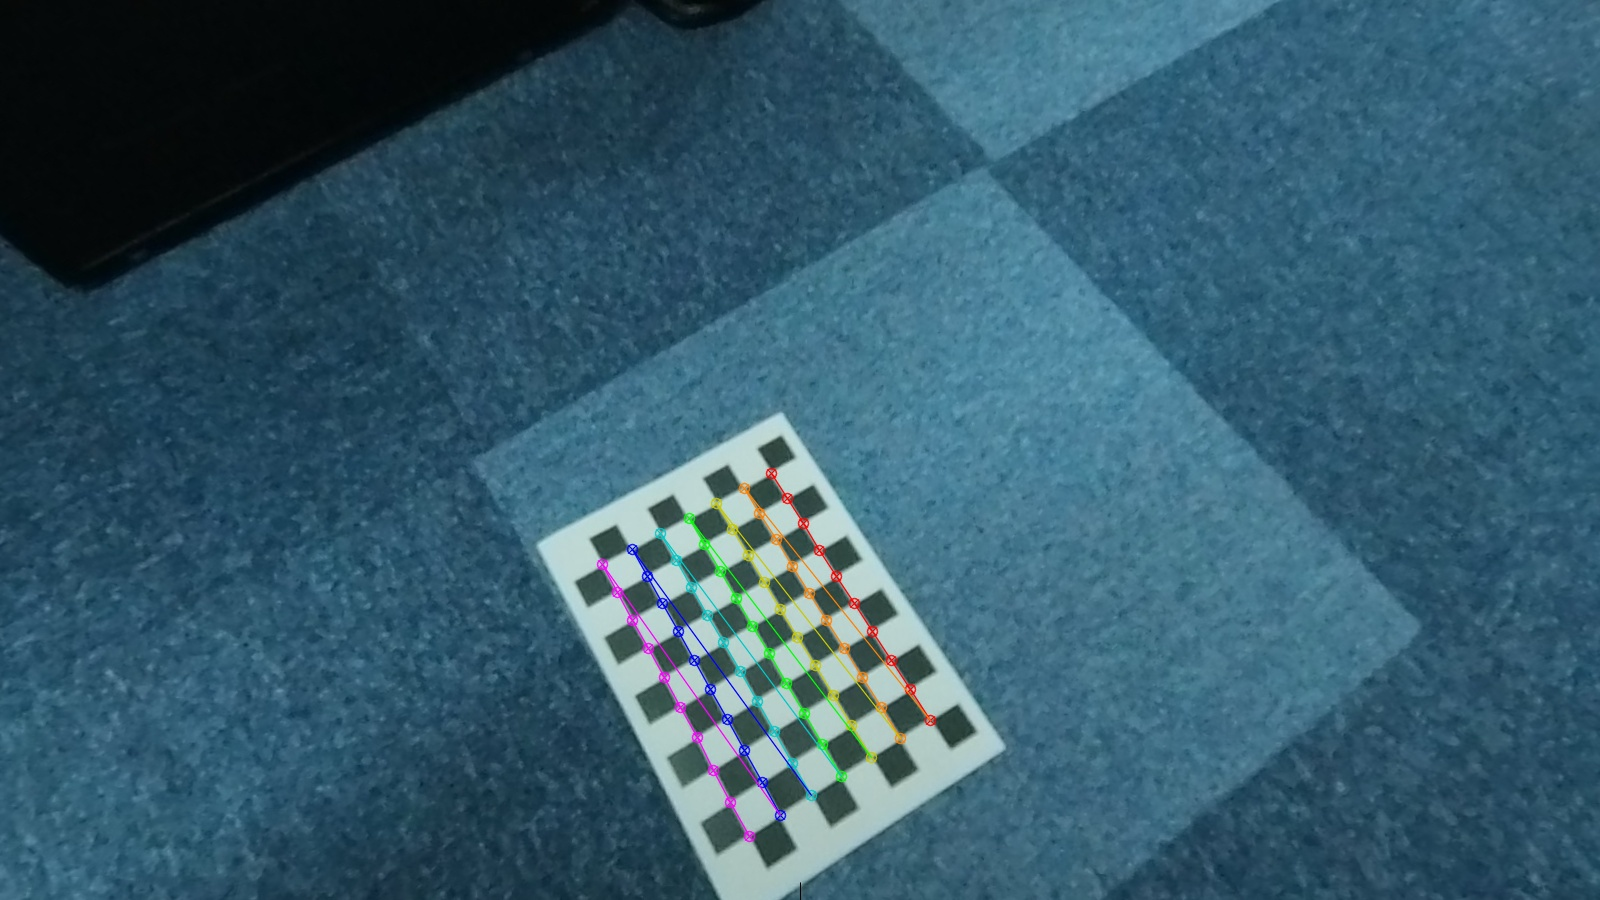
\includegraphics[keepaspectratio, width=0.4\linewidth]{figures/GetParam_result/1.jpg}&
      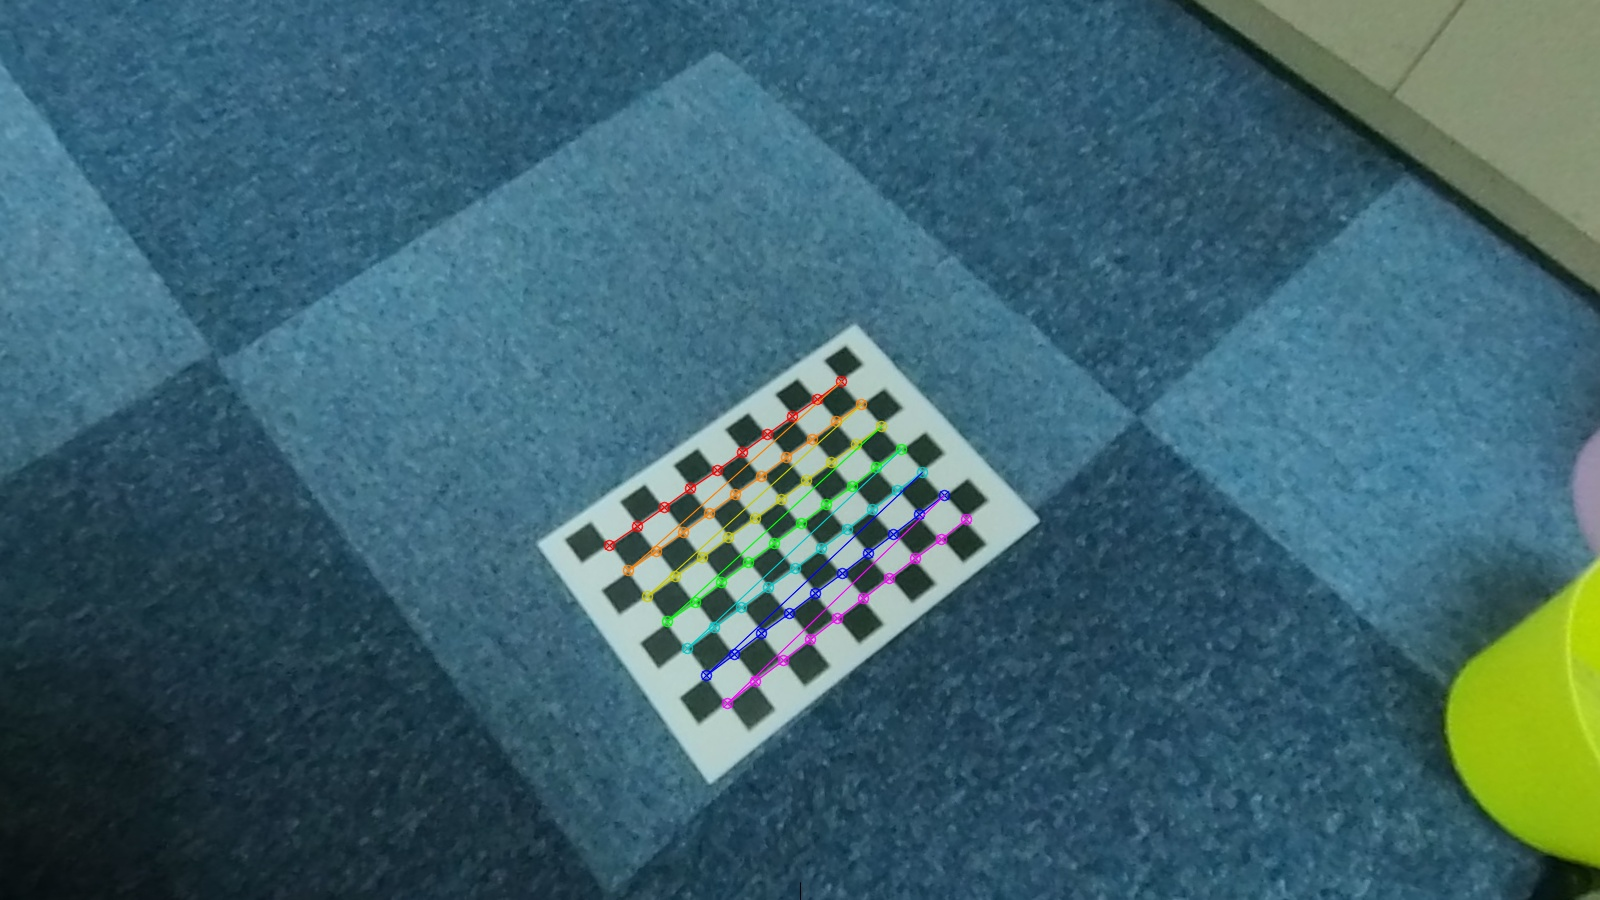
\includegraphics[keepaspectratio, width=0.4\linewidth]{figures/GetParam_result/5.jpg}\\
      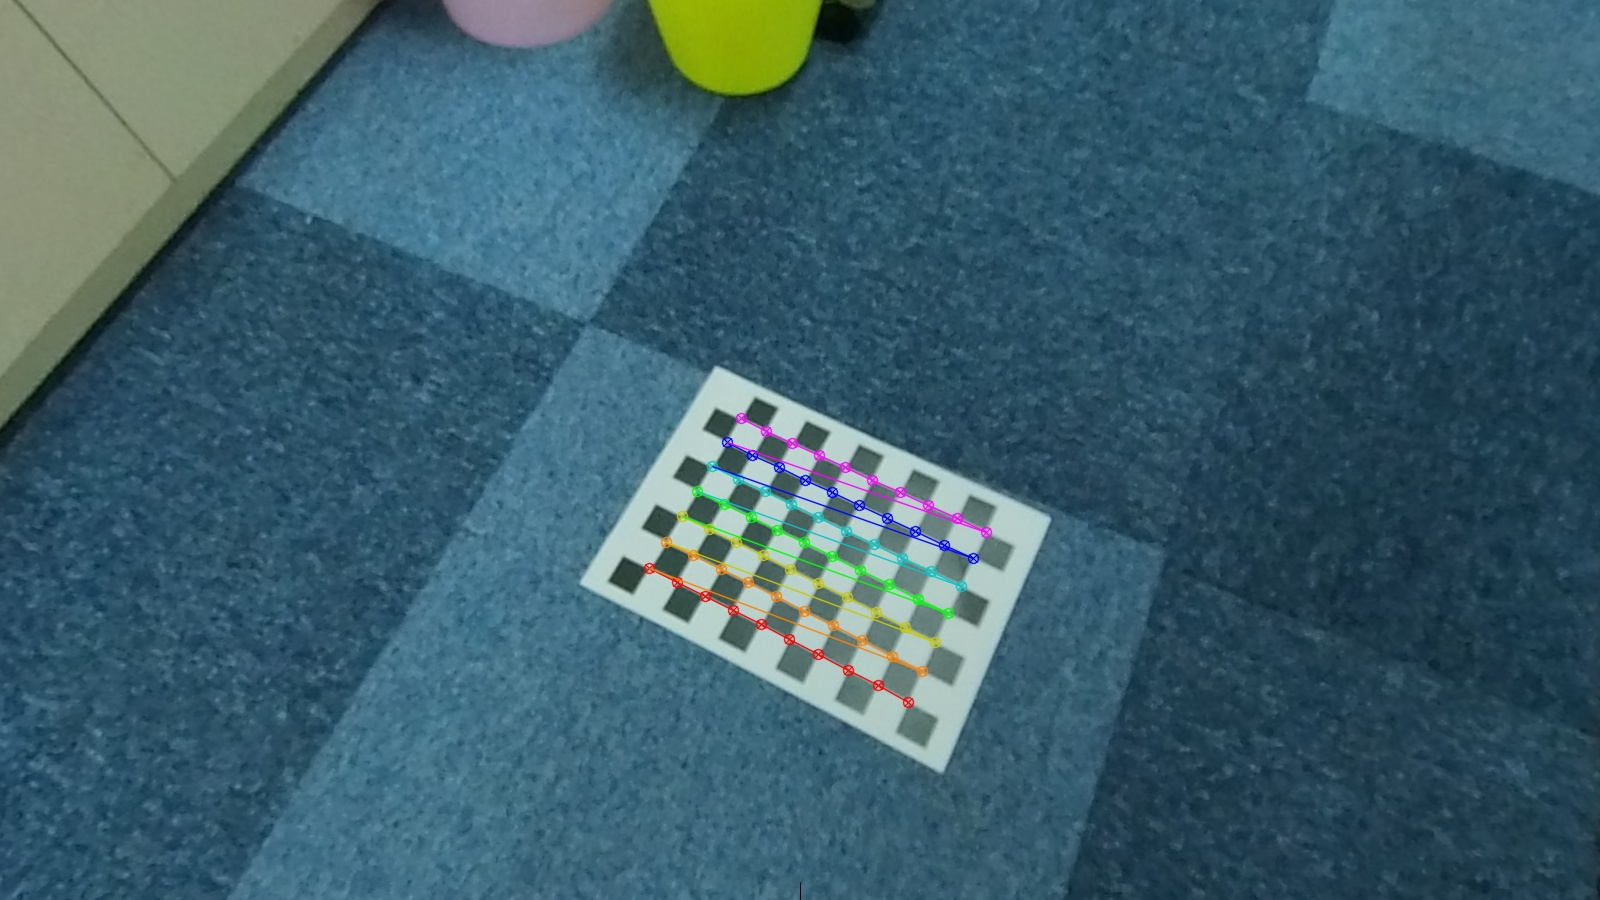
\includegraphics[keepaspectratio, width=0.4\linewidth]{figures/GetParam_result/9.jpg}&
      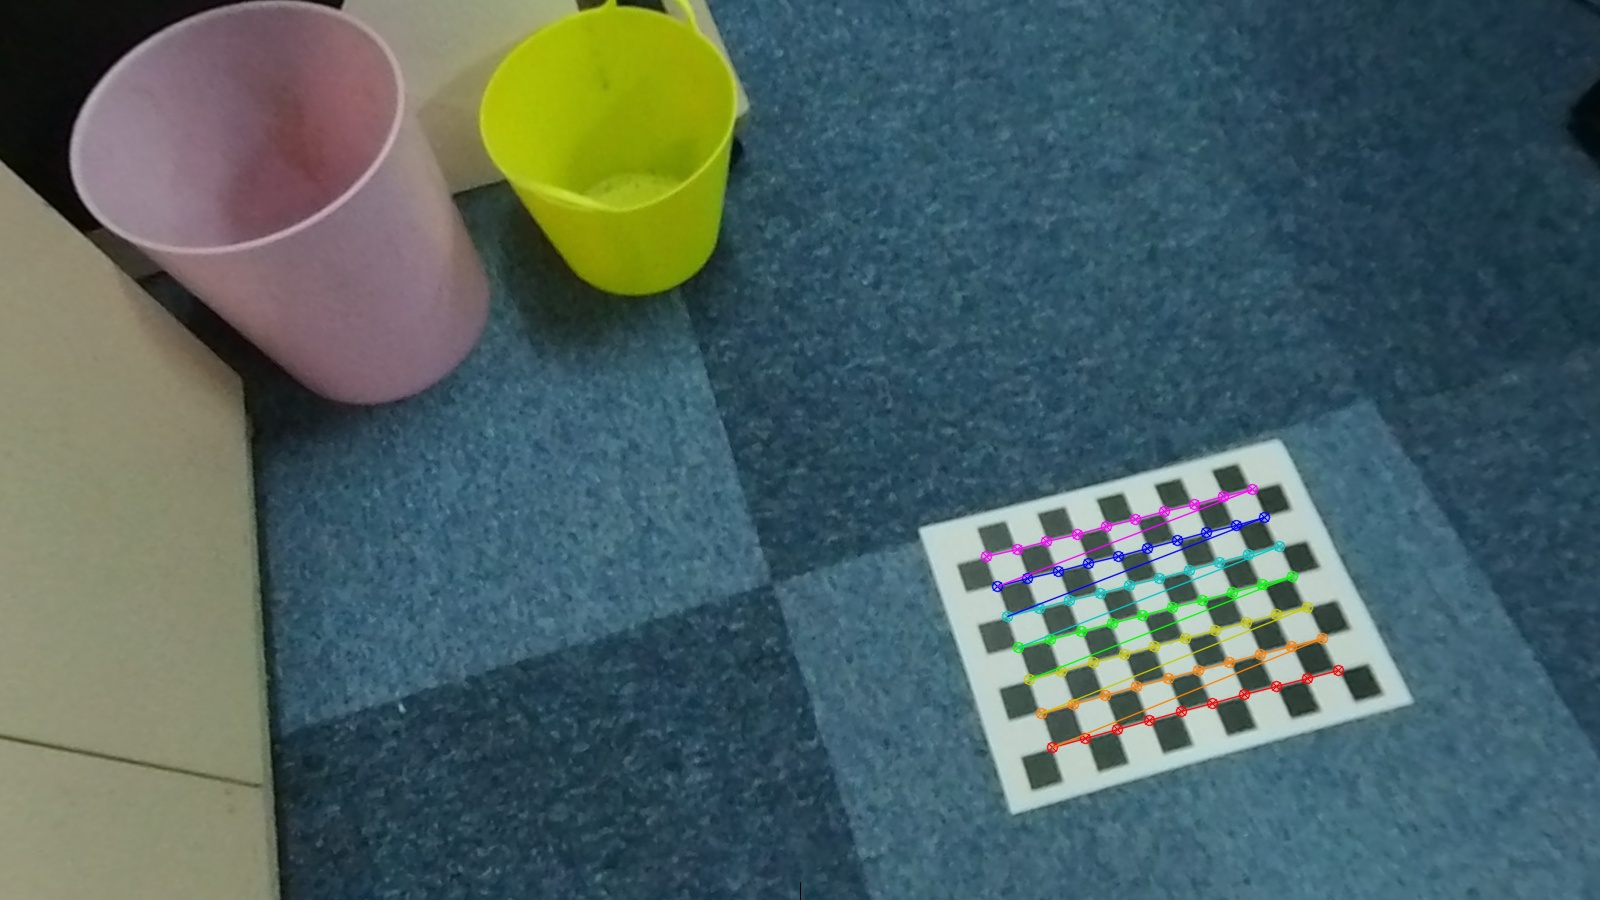
\includegraphics[keepaspectratio, width=0.4\linewidth]{figures/GetParam_result/13.jpg}\\
    \end{tabular}
  \end{center}
  \caption{キャリブレーション結果}
  \label{three}
\end{figure}
また、出力されたカメラの内部パラメータ行列$\MU$を以下に示す。
\begin{equation}
  \MU = 
  \begin{pmatrix}
    511.69918760786322 & 0.00000000000000 & 784.54139306531715 \\
    0.00000000000000 & 499.73234060481144 & 536.82834728101511 \\
    0.00000000000000 & 0.00000000000000 & 1.00000000000000 \\
  \end{pmatrix}
\end{equation}
これより、チェッカーボードの交点を検出し、カメラの内部パラメータが推測されていることがわかる。
また焦点距離$f_x=511.69918760786322$、$f_y=499.73234060481144$となったが、今回焦点距離は各軸共通なので$f_x$と$f_y$の平均を用いる。
\section{カメラ位置・姿勢推定の実行結果}
\subsection{入力}
直行射影の共線性と共面性を利用したカメラ姿勢の推定の際に必要な入力を以下に示す。
\begin{itemize}
  \item $\pU_a$:世界座標系で表現された空間点の座標
  \item $\vU_a$:$\pU_a$に対応する画像上の特徴点座標
  \item $\dU_a$:世界座標系で表現された直線$L_a$の方向ベクトル
  \item $\rU_a$:世界座標系で表現された直線$L_a$上の点の座標
  \item $\nU_a$:$L_a$に対応する画像上の直線のパラメータベクトル
  \item $\RU^0$:回転行列の初期値
  \item $thd$:収束に用いるしきい値
\end{itemize}
$\pU_a$は3次元モデルの頂点の座標の一部を用いる。ただし透視投影画像に映らない点については、空間点の座標として用いない。
3次元モデルについてはC棟エレベータ前の廊下のモデルを用いる。3次元モデルを\hyperref[one]{図\ref{one}}に示す。
\begin{figure}[!ht]
  \begin{center}
    \begin{tabular}{c}
      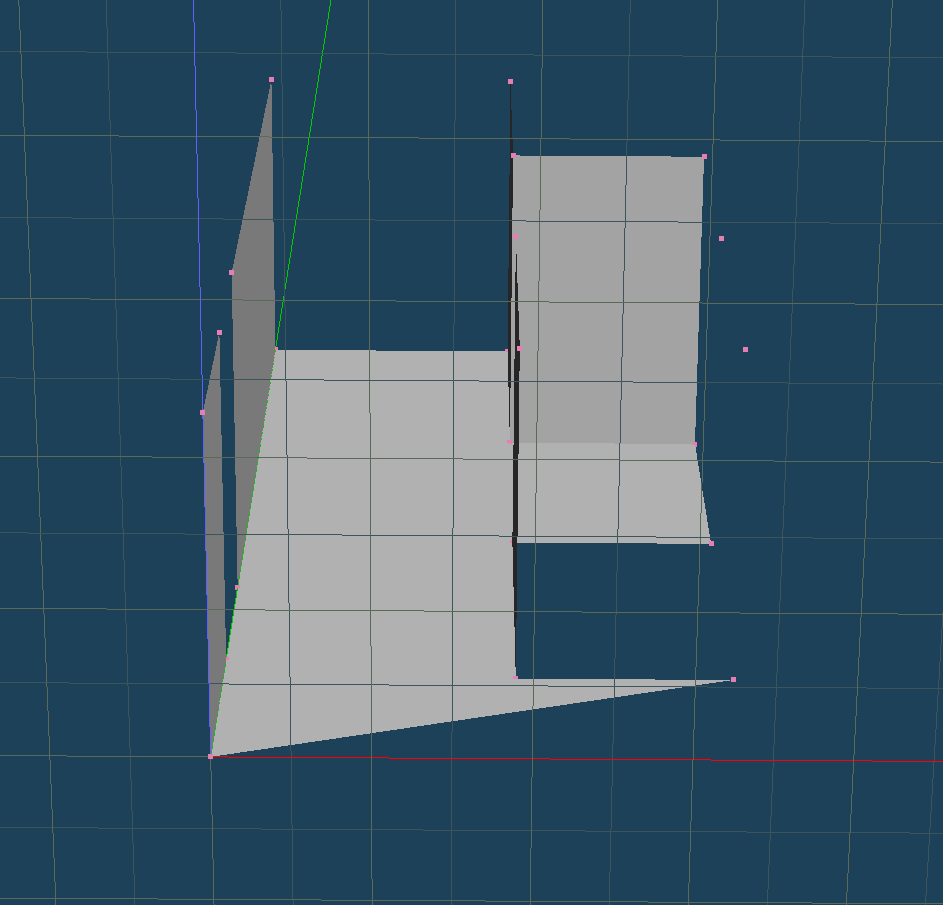
\includegraphics[keepaspectratio, scale=0.3]{figures/3dmodel.png}
    \end{tabular}
  \end{center}
  \caption{3dモデル}
  \label{one}
\end{figure}
\\
$\vU_a$は透視投影画像から手動で選択して用いる。透視投影画像を表示し$\pU_a$に対応する画像の座標をクリックする。
に追加される(\hyperref[two]{図\ref{two}})。
\begin{figure}[!ht]
  \begin{center}
    \begin{tabular}{c}
      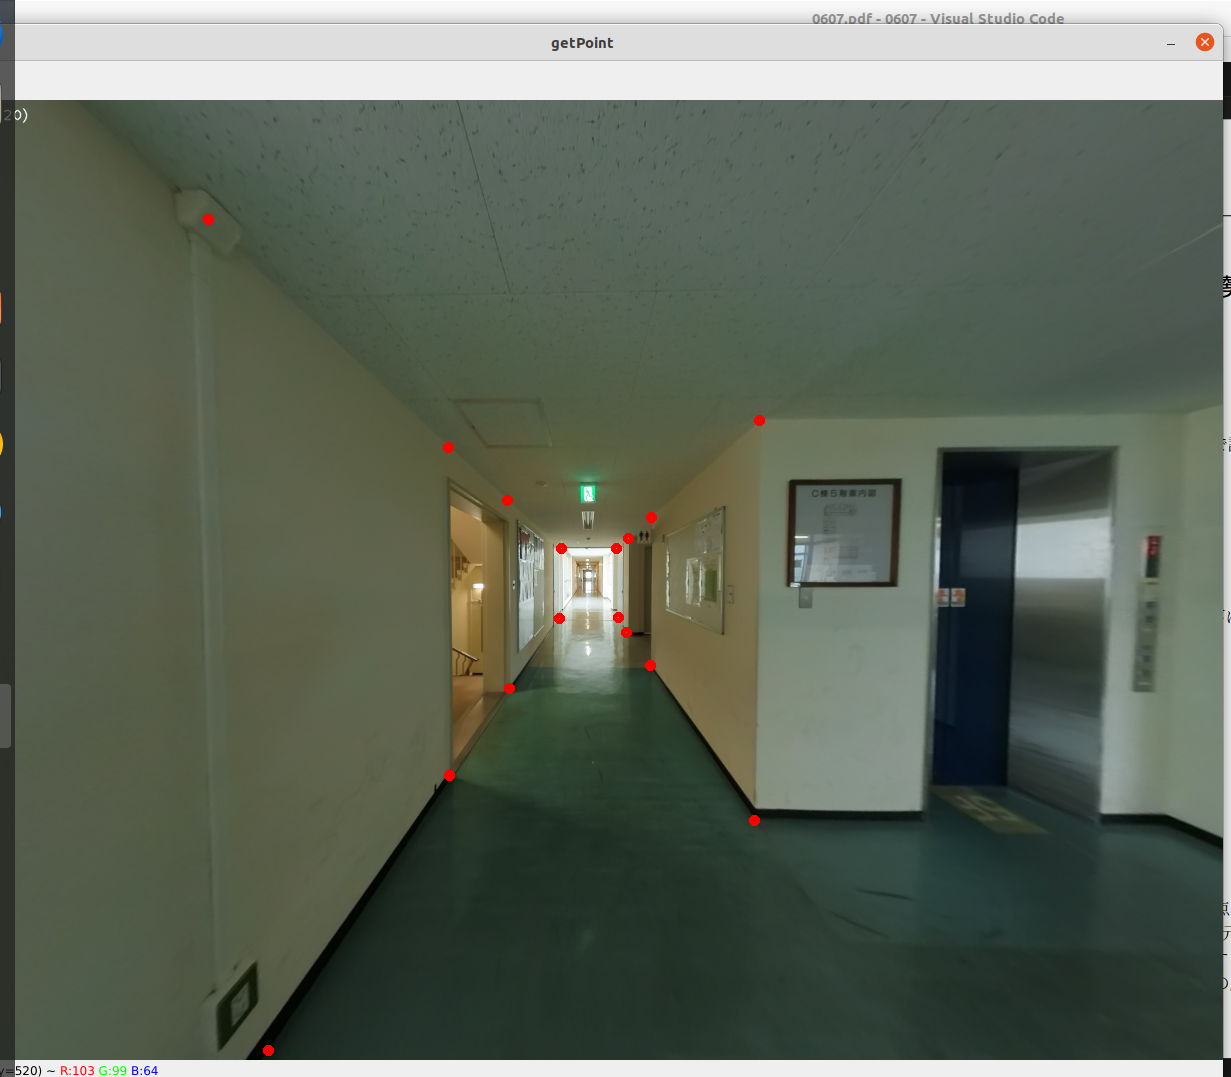
\includegraphics[keepaspectratio, scale=0.3]{figures/select_point.png}
    \end{tabular}
  \end{center}
  \caption{画像特徴点を選択}
  \label{two}
\end{figure}
また$\vU_a=(x_a,y_a,f)$で、$(x_a,y_a)$は光軸点を原点とした画像点の座標であるため、以下の式で平行移動する。
\begin{equation}
  x_a = x - frac{W}{2}, y_a = y - frac{H}{2}
\end{equation}
さらに、焦点距離$f$を座標の後ろに追加する必要がある。焦点距離$f$については、全方位カメラのキャリブレーションを行い計算した。
\\
$\dU_a={\dU_1,...,\dU_i,...}$については3次元モデルの頂点の座標の一部($\pU_a$で使用していない点)を用いて以下の式で求める。
\begin{equation}
  \dU_i = \frac{\pU_{i+1}-\pU_{i}}{|\pU_{i+1}-\pU_{i}|}
\end{equation}
\\
$\rU_a$については3次元モデルの頂点の座標の一部($\pU_a$で使用していない点)を用いる。
\\
$\nU_a={\nU_1,...,\nU_i,...}$については$\vU_a$の座標を用いて以下の式で用いる。
\begin{equation}
  \nU_i = \frac{\nU_{i+1}\times{\nU_{i}}}{|\nU_{i+1}\times{\nU_{i}}|}
\end{equation}
\\
$\RU^0$は世界座標毛糸カメラ座標系の関係から以下の行列を設定する。また、$thd=1.0^{-8}$とする。
\begin{equation}
  \RU^0 = 
  \begin{pmatrix}
    1 & 0 & 0 \\
    0 & 0 & -1 \\
    0 & 1 & 0 \\
  \end{pmatrix}
\end{equation}
\subsection{実行結果}
出力された回転行列$\RU$、及びカメラ位置$\cU$を以下に示す。
\begin{equation}
  \RU =
  \begin{pmatrix}
    0.99848126 & 0.01266343 & -0.05361733 \\
    -0.05432481 &  0.06440953 & -0.99644379 \\
    -0.00916493 & 0.9978432 & 0.06499965 \\
  \end{pmatrix}
\end{equation}
\begin{equation}
  \cU =
  \begin{pmatrix}
    0.99930194 \\
    -2.46764452 \\
    1.18038819 \\
  \end{pmatrix}
\end{equation}
回転行列、カメラ位置ともに想定したものと近い値が出力された。
また、収束にかかった計算回数は、平均して22回程度だった。

\section{今後の計画}
今後の計画として、計算されたカメラ運動行列を用いてテクスチャの貼り付けに早急に取り掛かりたい。
具体的には6月中にテクスチャを貼り付けた3次元モデルを完成させる。

%参考文献
\begin{thebibliography}{99}
\bibitem{bib_1} 菅谷保之,「直交射影の共線性と共面性を用いたカメラ姿勢の推定」
\end{thebibliography}

\end{document}
